\documentclass[UTF-8]{ctexbeamer}
\usetheme{Berkeley}
\usecolortheme{seahorse}

\usepackage{multimedia}
\usepackage{listings}
\usepackage{minted}
\usepackage{tikz}
\usepackage{textcomp}
\usepackage[normalem]{ulem}

\title{Proof Assistant - A 猫咪 Approach}

\author{喵喵}
\date{2022.3}

\begin{document}

\section{Intro}

\begin{frame}
  \titlepage
  \begin{center}
    
\includegraphics[width=.1\textwidth]{assets/float.png}
  \end{center}
\end{frame}

\begin{frame}
  \frametitle{Motivation}

  \pause
  \begin{figure}
    
\includegraphics[width=0.5\textwidth]{assets/doughnut.png}
    \caption{喵喵 embedded in $S^1 \times D^2$}
  \end{figure}
\end{frame}

\begin{frame}
  \frametitle{Motivation (Cont.)}

  \url{https://github.com/caotic123/PomPom-Language}
  
  \pause

  \vspace{1em}

  能否在 1000 行内使用 Rust 实现一个 Proof Assistant?

  \pause

  \begin{figure}
    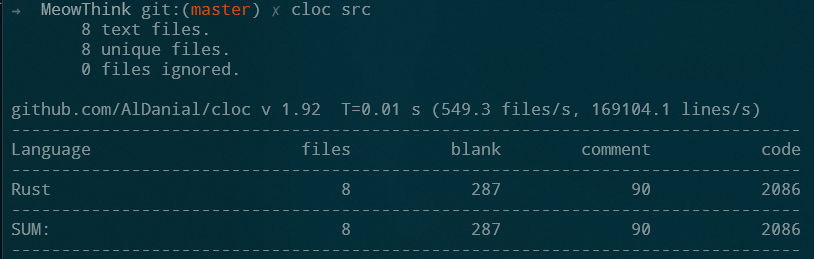
\includegraphics[width=\textwidth]{assets/cloc.png}
    \caption{"2000 LOC can (sort of)"}
  \end{figure}

  \url{https://github.com/CircuitCoder/MeowThink}

\end{frame}

\section{命题逻辑}

\begin{frame}
  \frametitle{直觉逻辑 - Why}
  
  \pause

  \begin{block}{中国民间数学家定理 (CFMT)}
    任意大于 2 的偶数,都可以表示成两个质数的和。
  \end{block}

  \pause

  \vspace{1em}

  \begin{columns}
    \begin{column}{0.5\textwidth}
      \centering
      "CFMT 和 ZFC 系统独立"

      \pause
      \vspace{0.5em}

      
\includegraphics[width=0.8\textwidth]{assets/le.png}
    \end{column}
    \pause
    \begin{column}{0.5\textwidth}
      \centering
      "CFMT 是哪个公理的结果?"

      \pause
      \vspace{0.5em}

      
\includegraphics[width=0.8\textwidth]{assets/bule.png}
    \end{column}
  \end{columns}
\end{frame}

\begin{frame}
  \frametitle{直觉逻辑 - How}

  经典逻辑:真值表是本质的。

  \begin{center}
  枚举 P, Q 取值可以证明 $ \overline{P \land Q} \rightarrow \overline{P} \lor \overline{Q} $
  \end{center}

  \pause

  直觉逻辑:推理,也就是\textbf{蕴含}($\rightarrow$)是本质的。

  \begin{center}
    如果已知 $P$, 已知 $P \rightarrow Q$, 可以证明 $Q$
  \end{center}

  \pause
  \vspace{1em}

  \begin{center}
    在直觉逻辑中,\textbf{排中律}和\textbf{双重否定去除}不自然成立。
  \end{center}
\end{frame}

\begin{frame}
  \frametitle{Curry-Howard 对应}
\end{frame}

\begin{frame}[fragile]
  \frametitle{We can prove stuff!}

  \begin{minted}{rust}
fn id<A>(a: A) -> A;

fn concat<A, B, C>(
  first: impl Fn(A) -> B,
  second: impl Fn(B) -> C
) -> impl Fn(A) -> C;

fn and_to_or<A, B>(and: (A, B)) -> Either<A, B> {
  Either::Left(and.0)
}
  \end{minted}
\end{frame}

\begin{frame}[fragile]
  \frametitle{We can prove stuff!}

  \begin{minted}{rust}
fn id<A>(a: A) -> A;

fn concat<A, B, C>(
  first: A -> B,
  second: B -> C
) -> (A -> C);

fn and_to_or<A, B>(and: A × B) -> (A + B) {
  Left(and.first)
}
  \end{minted}
\end{frame}

\begin{frame}[fragile]
  \frametitle{We can prove stuff!}

  \begin{block}{LEM Irrefutable}
  $$
  \neg \neg (P \lor \neg P)
  $$
  \end{block}

  \pause
  \vspace{2em}

  \begin{minted}{rust}
fn lem_irrefutable<P>(
  lem_false: (P + (P -> !)) -> !
) -> ! {
  let p_to_false: P -> !
    = |p: P| lem_false(Left(p));
  lem_false(Right(p_to_false))
}
  \end{minted}
\end{frame}

\begin{frame}[fragile]
  \frametitle{Wait a minute...}

  \pause

  \begin{minted}{rust}
    fn bad<T>(t: T) -> ! {
      loop { /* Meow */ }
    }

    fn worse<T>(t: T) -> ! {
      // Meow meow
      worse(t)
    }
  \end{minted}

  \pause

  \vspace{1em}

  \begin{block}{函数}
    在数学中为两不为空集的集合间的一种对应关系:
    
    输入值集合中的每项元素皆能对应\textbf{唯一一项}输出值集合中的元素。
  \end{block}
\end{frame}

\begin{frame}
  \frametitle{Totality checker}

  递归必须结束。

  \pause

  \vspace{1em}

  检查循环是否终止比较麻烦。
  
  \pause
  
  循环可以用递归替代 - 不允许循环。
\end{frame}

\section{谓词逻辑}

\begin{frame}
  \frametitle{一阶逻辑?}

  我们如何表示谓词?

  \begin{block}{命题 Even}
    $$
    \text{n 是自然数}, Even(n) \mapsto \text{n 是个偶数}
    $$

    \pause
    \vspace{0.5em}

    $$
    Even: \text{自然数} \rightarrow \text{命题}
    $$

    \pause
    \vspace{0.5em}

    \begin{center}
      \texttt{P: Nat -> Type}
    \end{center}
  \end{block}
\end{frame}

\begin{frame}
  \frametitle{\texttt{Data -> Type}??}

  \pause

  \texttt{Type -> Type}: 泛型 (Generic)

  \pause

  \texttt{Constant -> Type}: Const Generic

  \pause

  \texttt{Data -> Type}: Dependent Typing
\end{frame}

\begin{frame}
  \frametitle{Dependent Typing}
\end{frame}

\begin{frame}[fragile]
  \frametitle{类型表示}

  \begin{minted}{rust}
    fn id<A>(a: A) -> A;
  \end{minted}

  \pause

  \begin{center}
    \texttt{id<A>: A -> A}

    \pause
    \vspace{1em}

    \texttt{id: (A: Type) -> A -> A}
  \end{center}
\end{frame}

\begin{frame}
  \frametitle{量词}

  \pause
  $$
  \forall, \exists
  $$
\end{frame}

\begin{frame}[fragile]
  \frametitle{We can prove (more) stuff!}

  \begin{block}{Axiom of Choice...?}
  如果对于一组集合 S(i) 中的每一个,都可以选出来一个元素 s 满足 P(i, s),那么存在一个选择函数,从每个 S(i) 中选出一个,使得每个选择的结果都满足谓词 P
  \end{block}

  \pause

  $$
  \begin{aligned}
  &\forall i \in I, \exists s \in S(i), P(i, s) \\
  &\rightarrow \\
  &\exists f: ((i: I) \rightarrow S(i)) \\
  &\forall i \in I, P(i, f(i))
  \end{aligned}
  $$
\end{frame}

\begin{frame}[fragile]
  \frametitle{We can prove (more) stuff!}

  \begin{minted}{rust}
fn not_exactly_choice(
  Index: Type,
  Set: Index -> Type,
  Pred: Index -> Set -> Type,

  all_has_elem: (
    (i: Index)
    -> ((s: Set(i)) × Pred(i, s))
  )
) -> (
  (f: (i: Index) -> Set(i))
  × ((any: Index) -> Pred(any, f(any)))
);
  \end{minted}
\end{frame}

\begin{frame}
  \frametitle{Equality}
\end{frame}

\begin{frame}
  \frametitle{What is \texttt{Type}}
\end{frame}

\section{归纳}

\section{公理}

\begin{frame}
  \frametitle{公理}
\end{frame}

\begin{frame}
  \frametitle{排中律}
\end{frame}

\begin{frame}
  \frametitle{外延性}
\end{frame}

\end{document}
